\documentclass[12pt]{article}
\usepackage[utf8]{inputenc}
\usepackage[english]{babel}
\usepackage{geometry}
\usepackage{listings} % for code snippets
\usepackage{xcolor}
\usepackage{graphicx}
\usepackage{titlesec}

% page setup and spacing
\geometry{a4paper, margin=0.75in}
\setlength{\parindent}{1em}
\setlength{\parskip}{1em}
\renewcommand{\baselinestretch}{1.0}

% colors for code snippet
\definecolor{codegreen}{rgb}{0,0.6,0}
\definecolor{codegray}{rgb}{0.5,0.5,0.5}
\definecolor{codepurple}{rgb}{0.58,0,0.82}
\definecolor{backcolour}{rgb}{0.95,0.95,0.92}

% code snippet styling
\lstdefinestyle{mystyle}{
    backgroundcolor=\color{backcolour},   
    commentstyle=\color{codegreen},
    keywordstyle=\color{magenta},
    numberstyle=\tiny\color{codegray},
    stringstyle=\color{codepurple},
    basicstyle=\ttfamily\footnotesize,
    breakatwhitespace=false,         
    breaklines=true,                 
    captionpos=b,                    
    keepspaces=true,                 
    numbers=left,                    
    numbersep=5pt,                  
    showspaces=false,                
    showstringspaces=false,
    showtabs=false,                  
    tabsize=2
}
\lstset{style=mystyle}

\title{ESOF 322: Homework 4}
\author{River Kelly and Peyton Dorsh}
\date{November 4, 2021}

\begin{document}
\maketitle
\newpage
\section*{Exercise 1 (15 pts)}
\subsection*{UML Class Diagram}
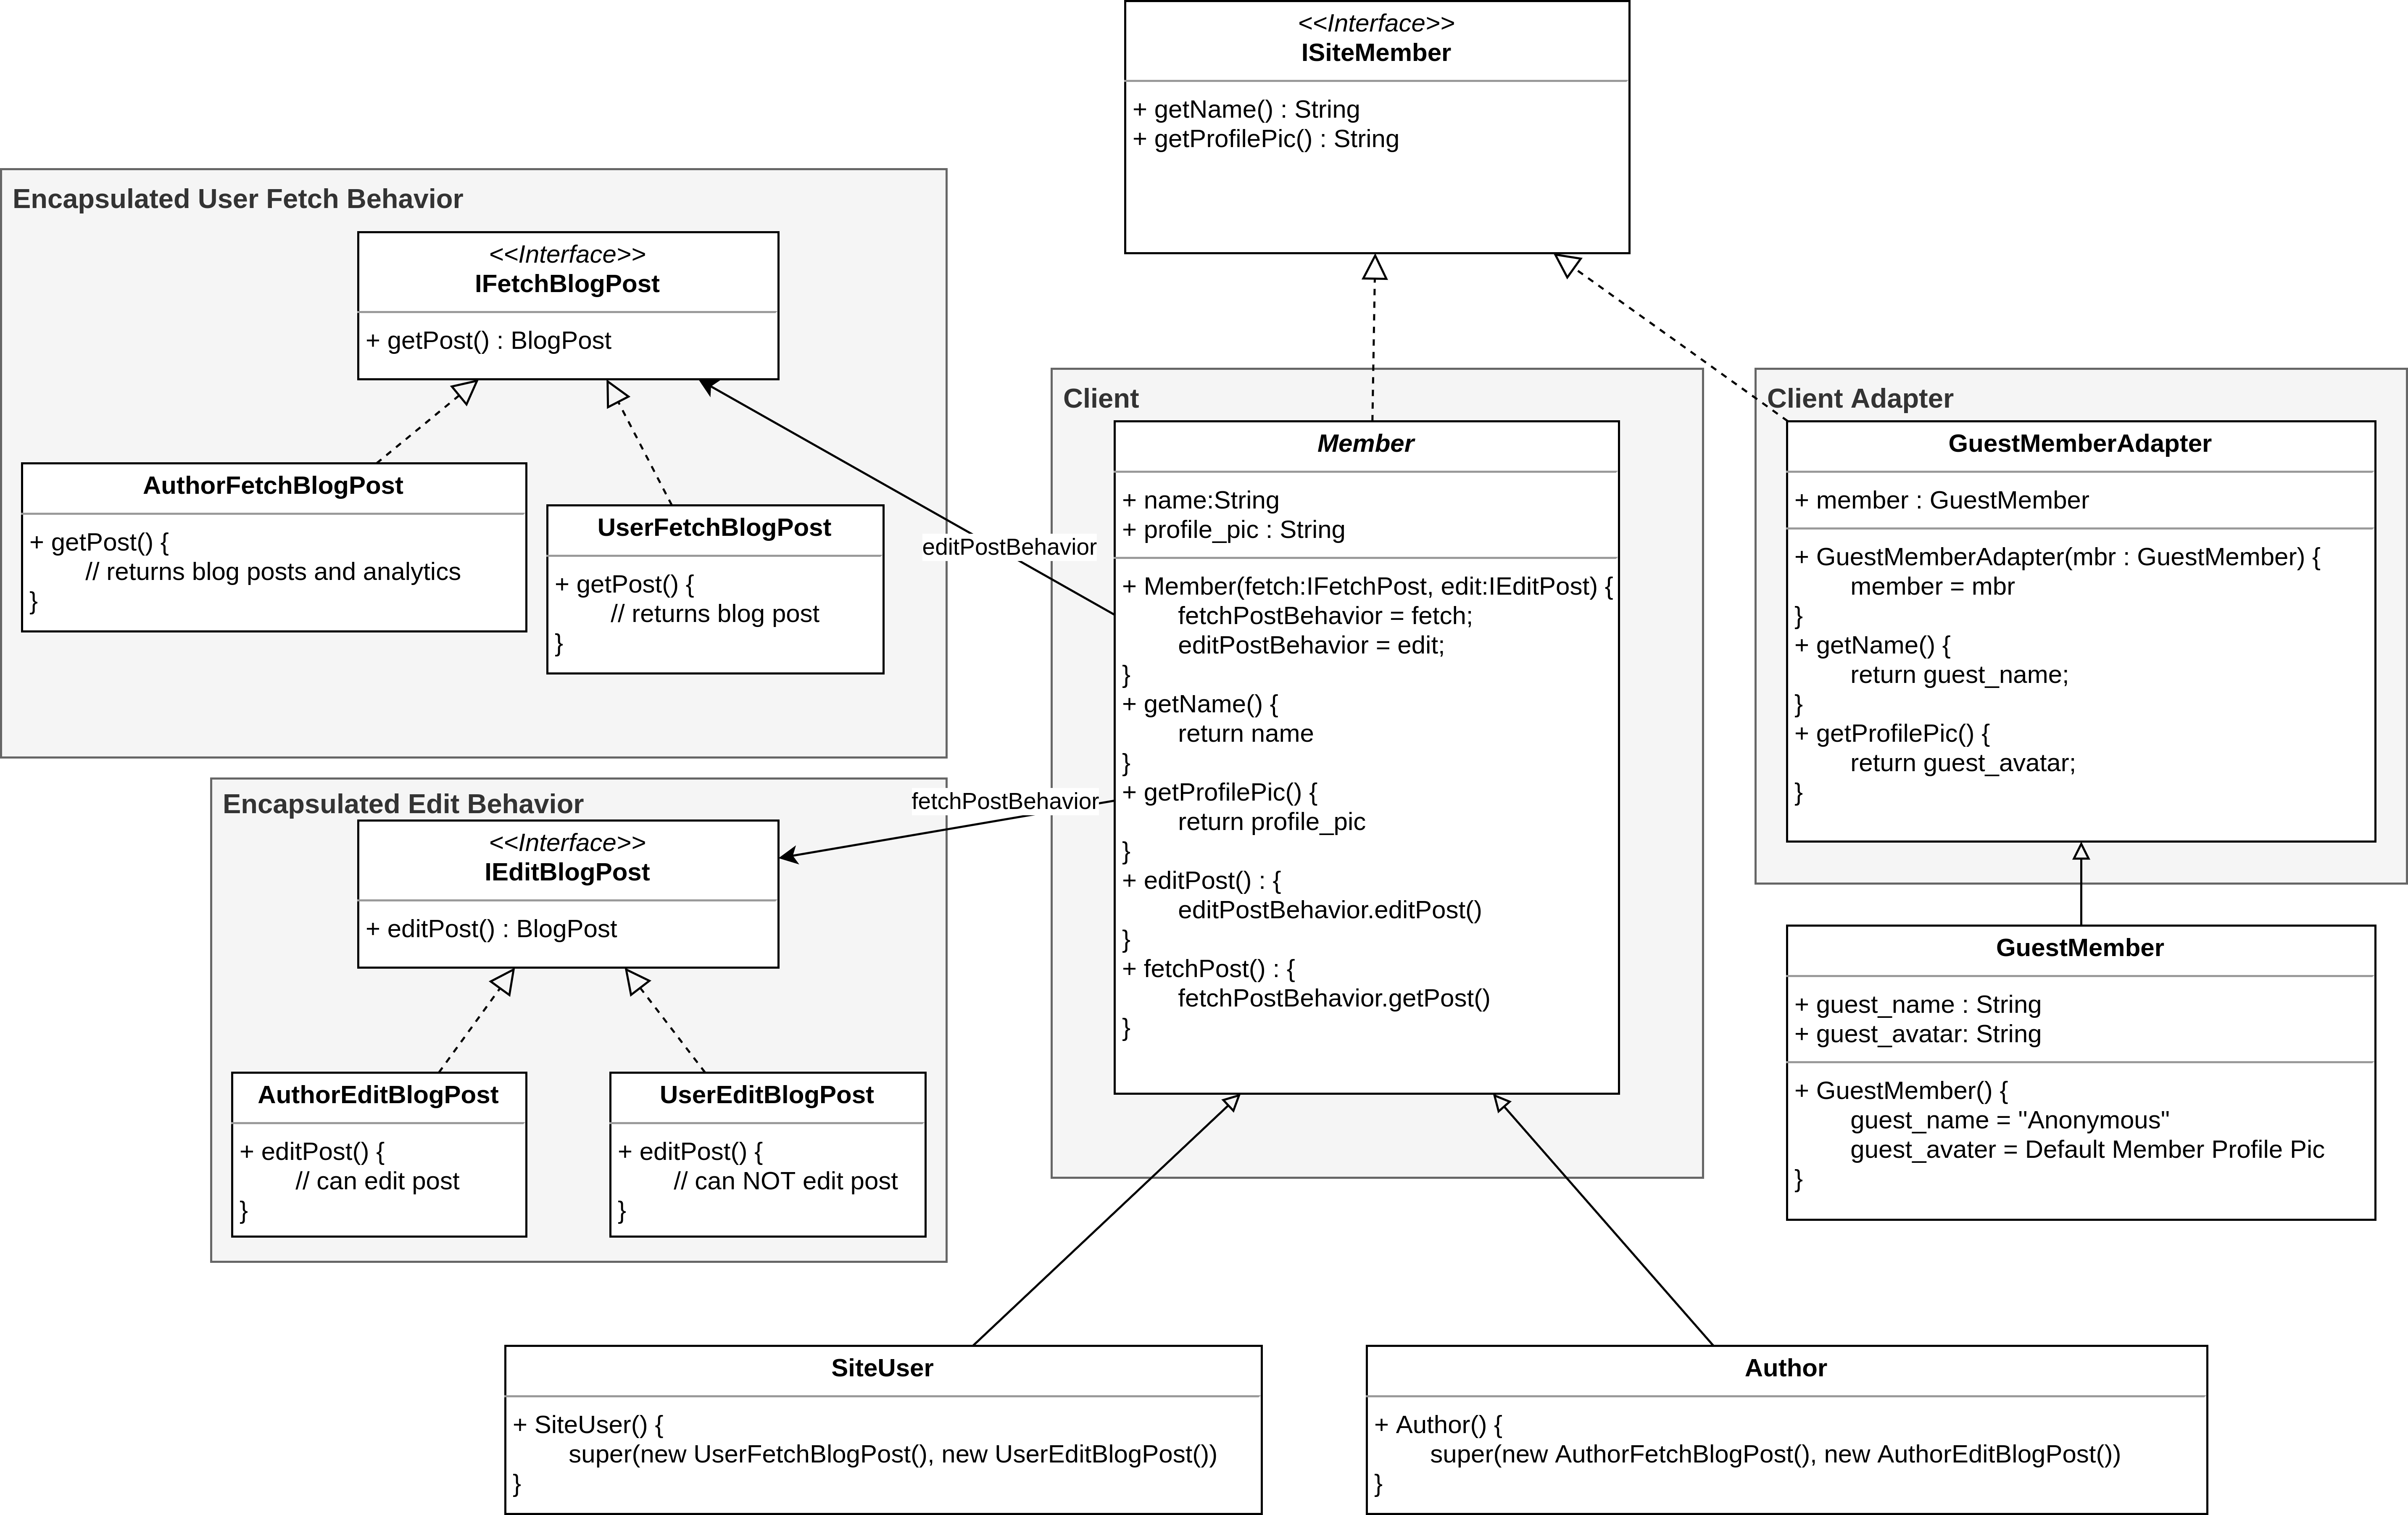
\includegraphics[width=\linewidth]{UML-Class-Diagram.png}
\subsection*{Strategy Sequence Diagram}
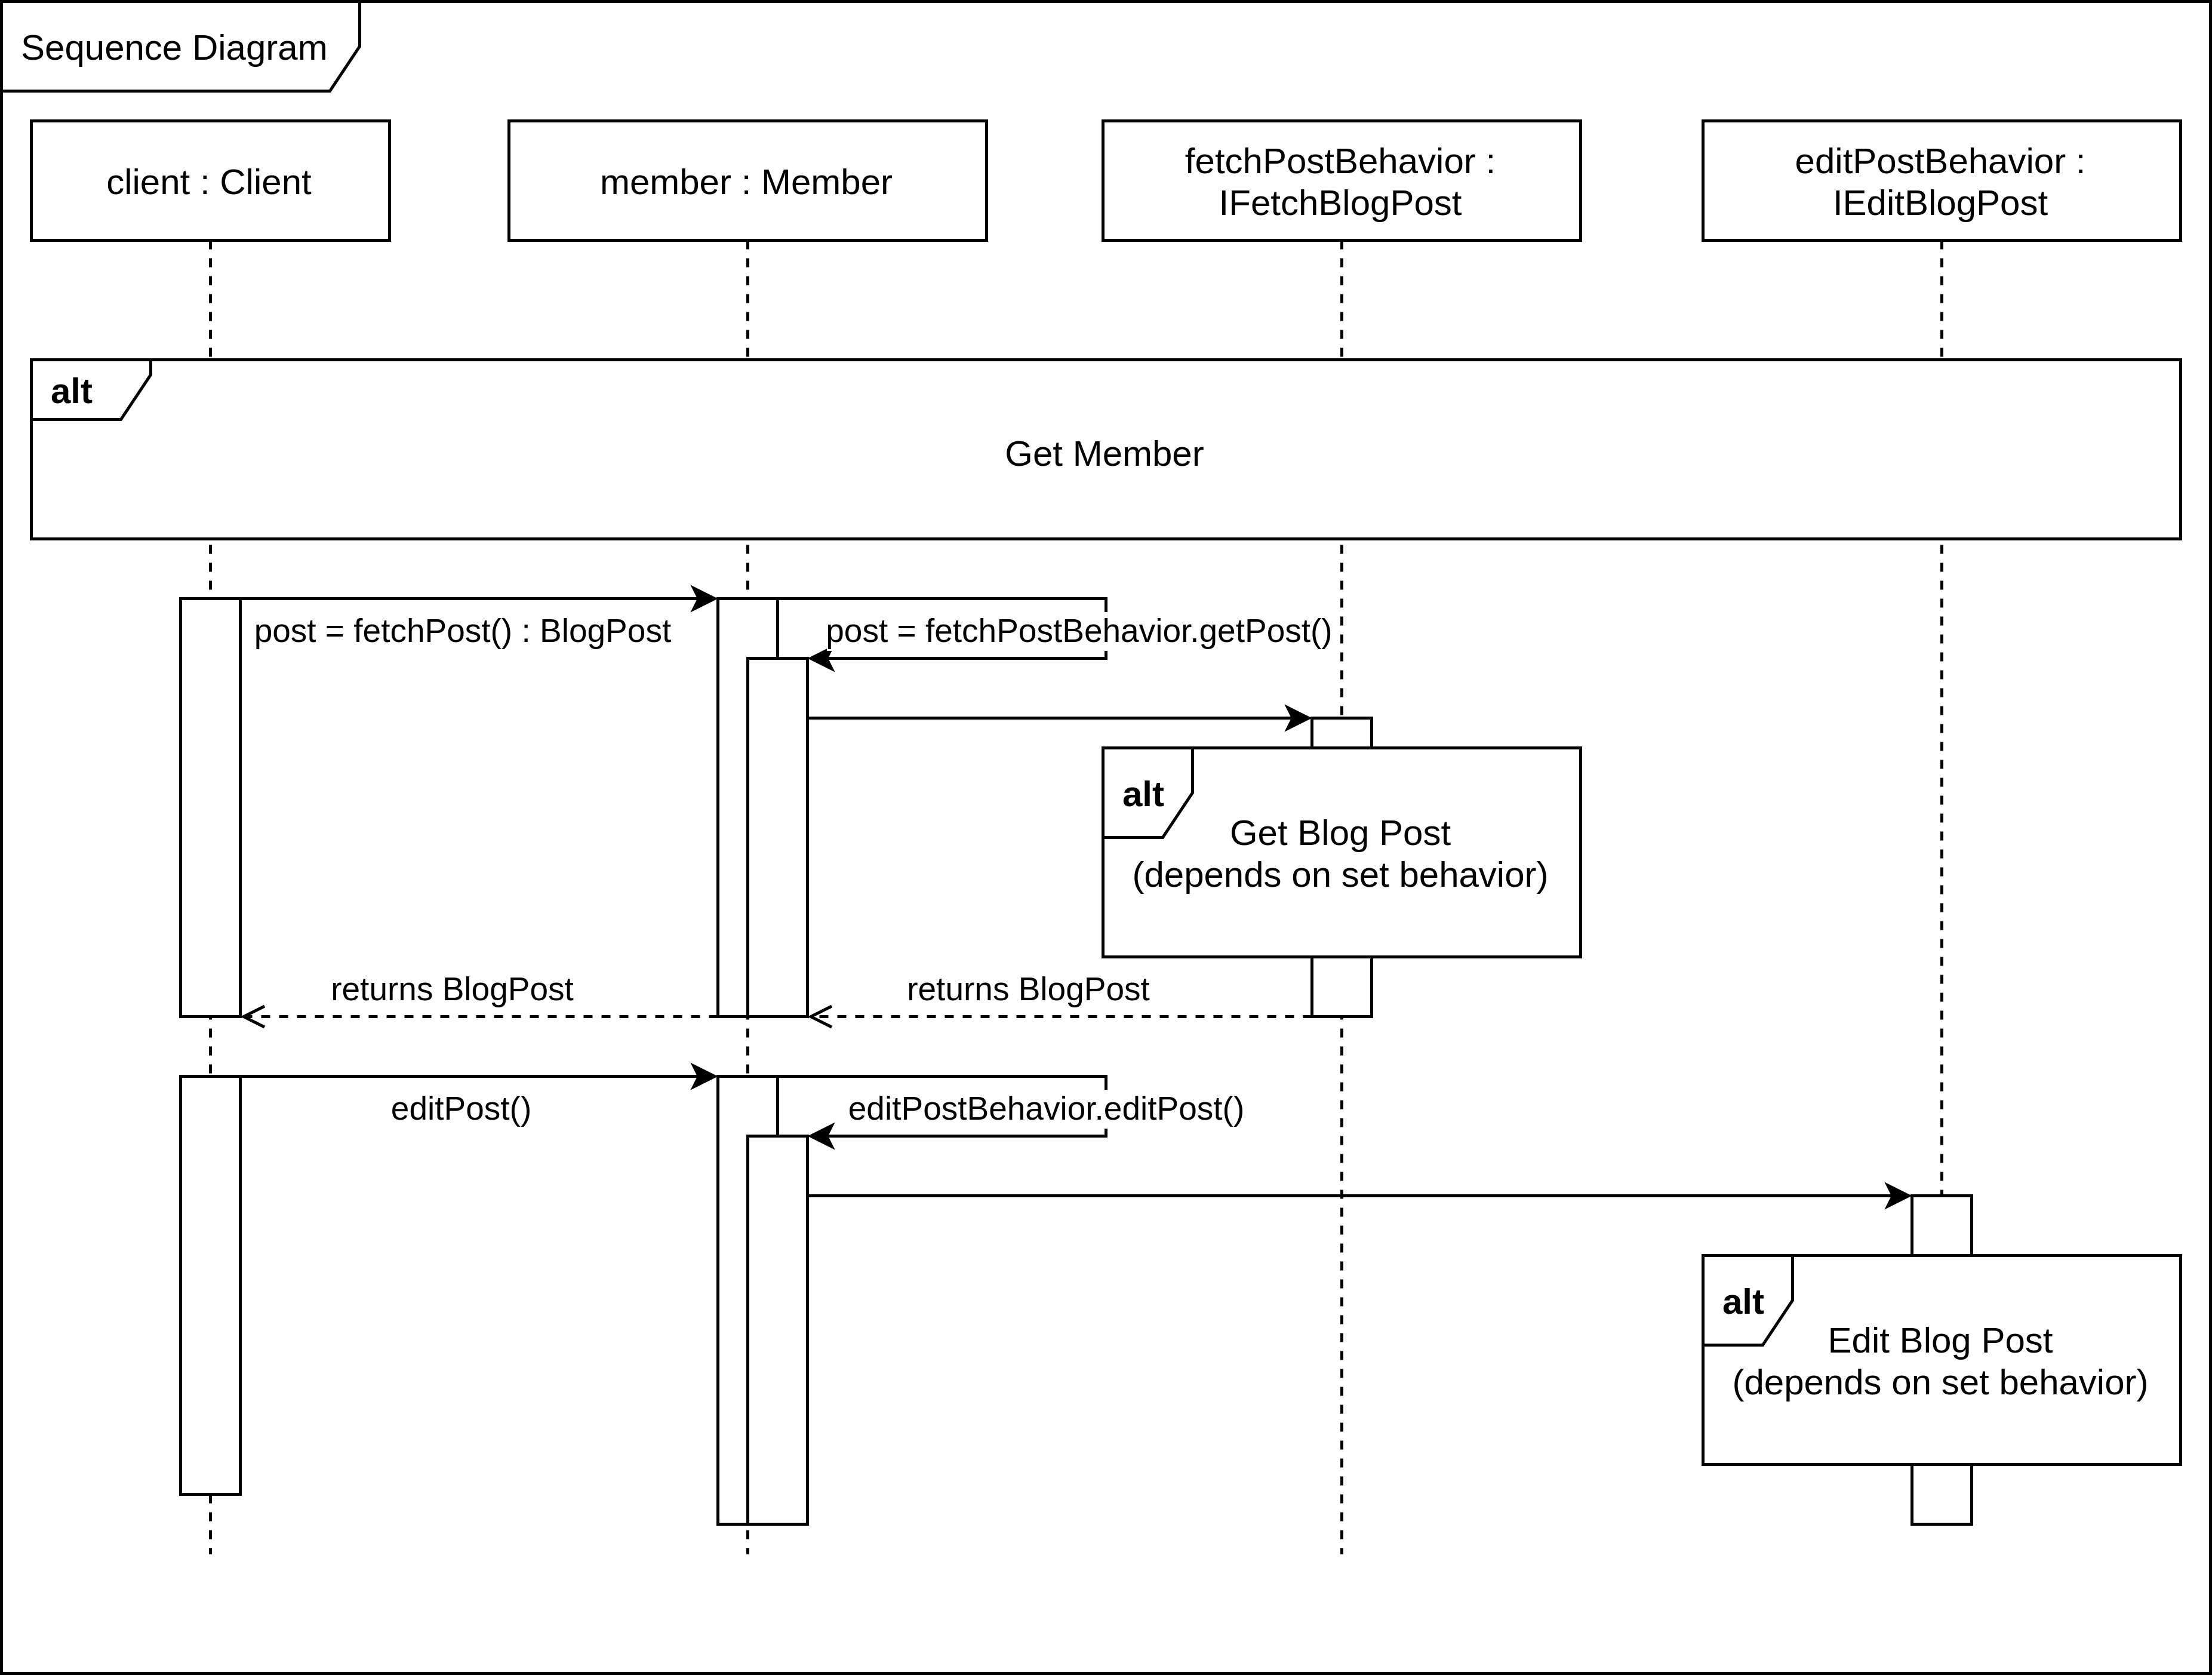
\includegraphics[width=\linewidth]{Sequence-Diagram-Strategy.png}
\newpage
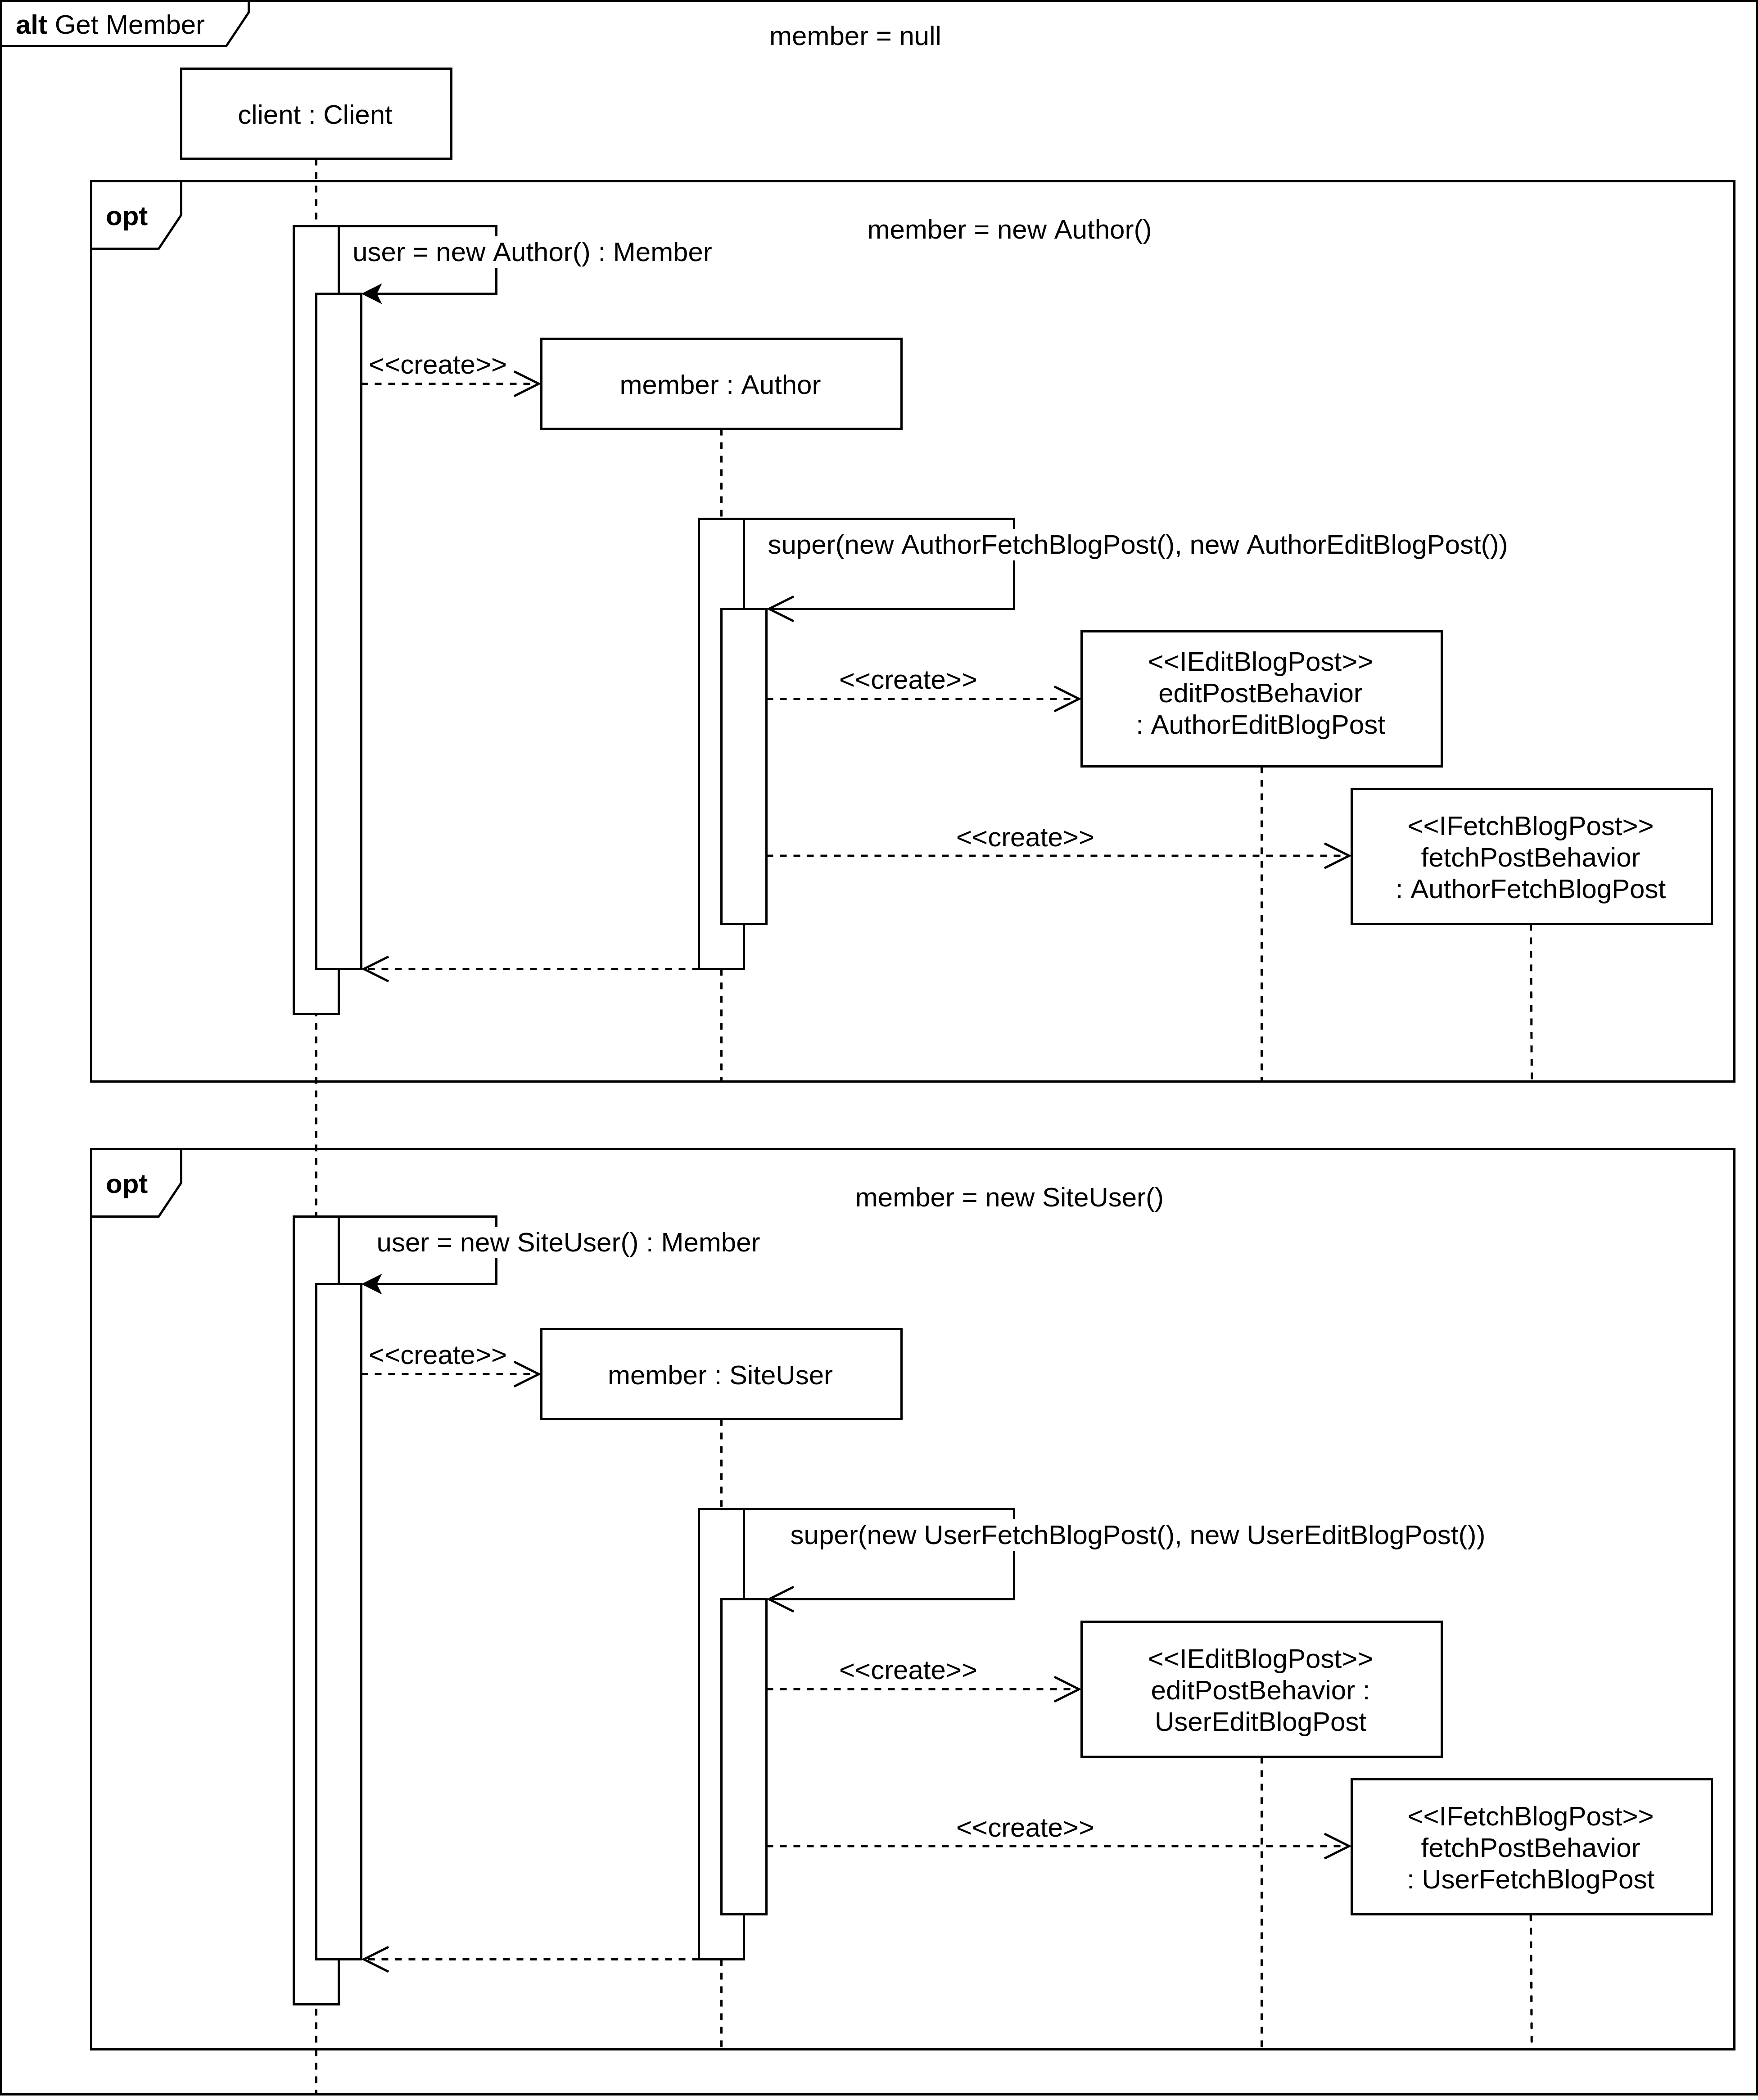
\includegraphics[width=\linewidth]{Sequence-Diagram-Strategy-1.png}
\newpage
\subsection*{Adapter Sequence Diagram}
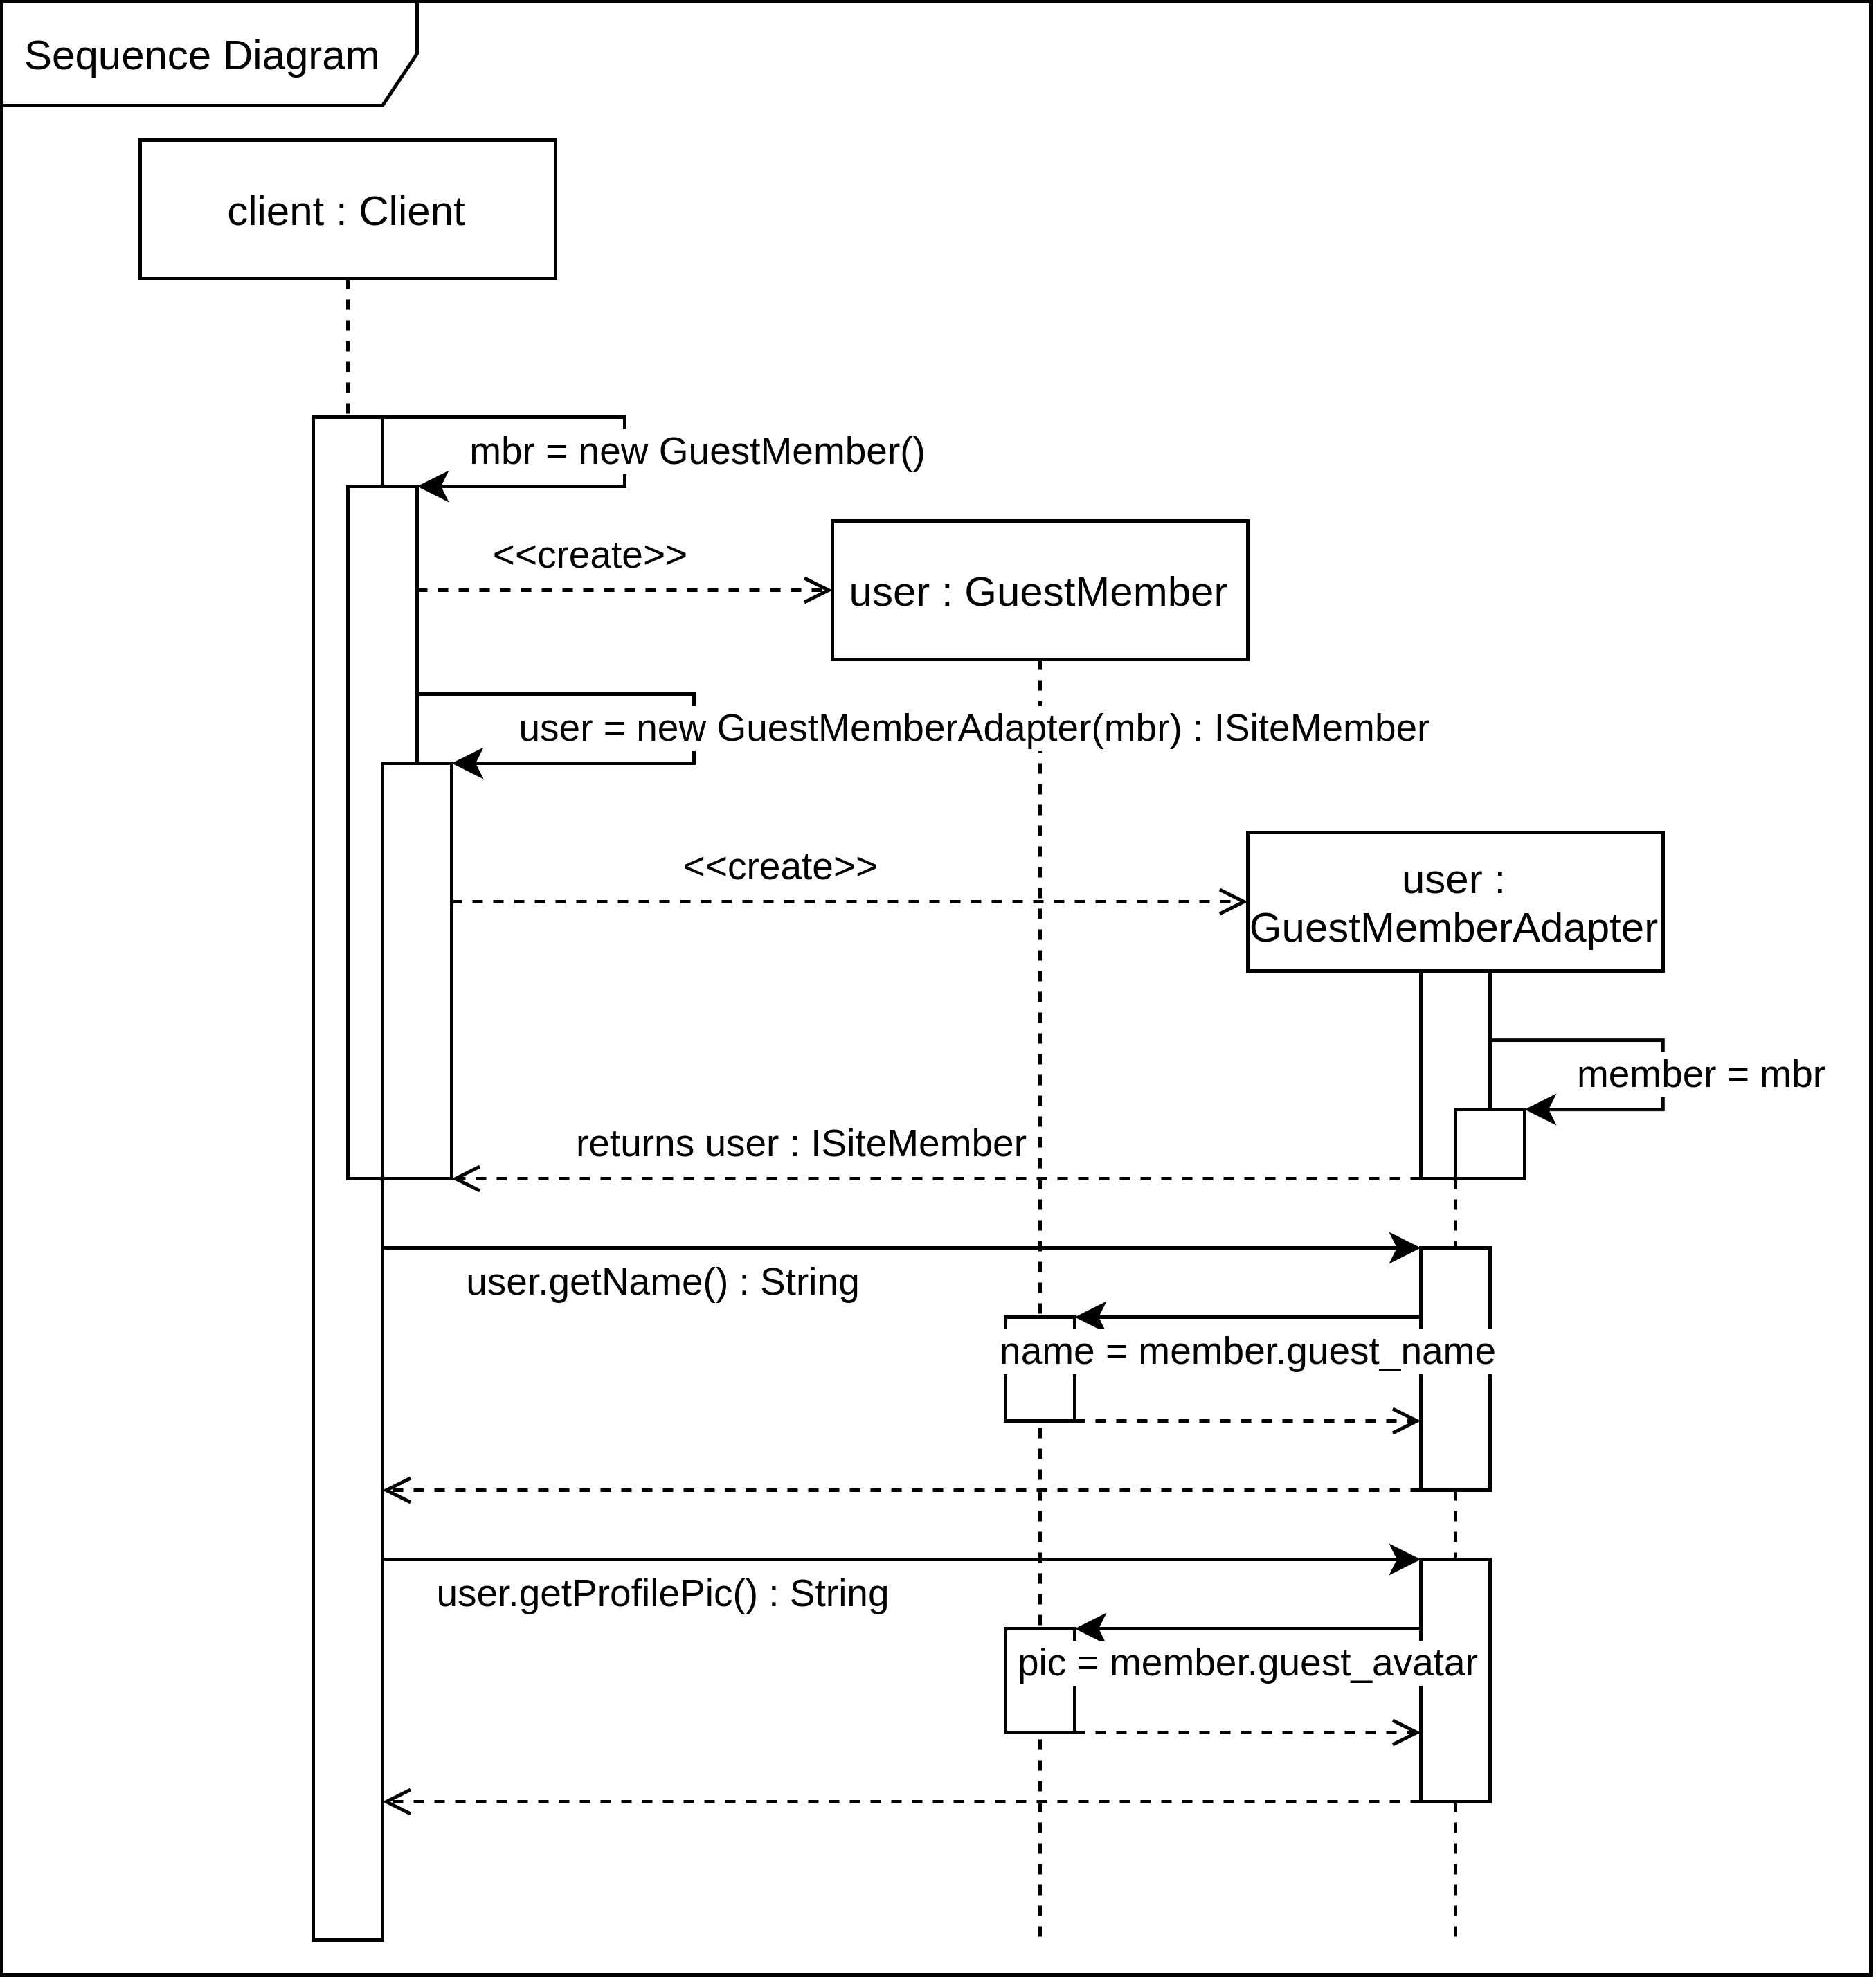
\includegraphics[width=\linewidth]{Sequence-Diagram-Adapter.png}
\newpage
\section*{Exercise 2 (10 pts)}
\begin{enumerate}
    \item Man in the Middle attacks is where a third party secretly listens in on communications between two other parties. An example is a foreign spy agency intercepting messages meant for an important government official and then forwarding those messages while pretending to be the original sender. This would let them secretly listen in on highly classified information or even stop messages from reaching the intended receiver.
    \item Cross-Site Scripting attacks are when a party sends a script message to a website that is then executed by the server. An example would be sending a script that quietly steals login information for amazon accounts by sending the information to themselves before letting the user log in. This party could use the information to order products using stolen credit card information or steal AWS credits for crypto mining.
\end{enumerate}

\end{document}
